\documentclass{article}
\usepackage[utf8]{inputenc}

\title{PS6 Holt}
\author{richard.n.holt}
\date{February 2019}

\usepackage{natbib}
\usepackage{graphicx}

\begin{document}

\maketitle

\section{Steps for Data Scraping and Cleaning}
I used data from the movie website IMDB. I thought about doing this because of the drama surrounding the Oscar's, and I wanted to see what the most popular movies of 2018 had in common.

I first looked at the block of information for each movie and determined what pieces of information would be important for determining popularity. I used the genre of the movie to test how well the variables correlate.

I wanted to use the rankings of the movies but I could not find a way to substring the number alone without creating two cases of each. I also had trouble with trying to get the ratings of the movie from the third party website, which I cannot explain at all. I also had a very difficult time using substring to clean the titles of the movies, and I am wondering if there is a good tutorial for using substring to locate characters within strings and use those as markers.

Jk, I got the rankings of the movies and I decided to also use the data about their runtime. Maybe people don't like watching longer movies. I also managed to clean up the titles after extensive research about string functions.

\section{Data Visualization}

The three graphs convey interesting information about the top films on IMDB. Graph A is a histogram of runtimes for the different movies. Despite the relatively small sample, we see a fairly normal distribution of runtimes, indicating that runtimes aren't very significant in determining a movie's popularity.

\begin{figure}[h!]
\centering
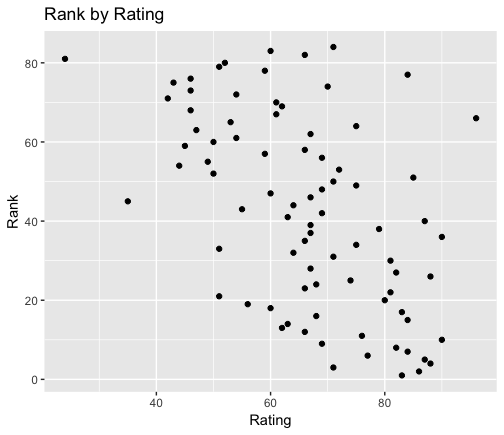
\includegraphics[scale=.5]{PS6a_Holt}
\caption{Runtimes}
\label{fig:PS6a_Holt}
\end{figure}

The second test of this relationship is shown in Graph B. This graph plots the relationship between runtimes and rating. The ratings seem to be completely unrelated to the runtime, meaning that the runtime has little to no bearing on whether people enjoyed a movie, at least as it relates to the most popular movie.

\begin{figure}[h!]
\centering
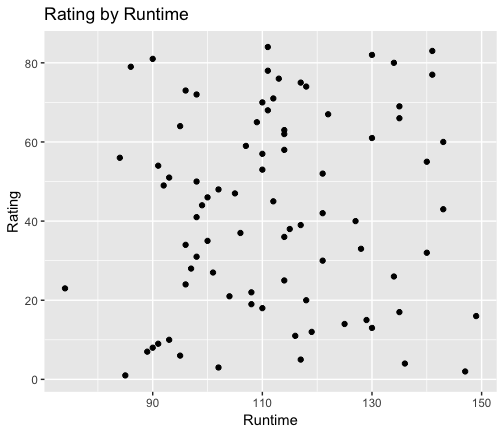
\includegraphics[scale=.5]{PS6b_Holt}
\caption{Runtimes v. Ratings}
\label{fig:PS6b_Holt}
\end{figure}

The third graph is the most interesting to me. I noticed that there were movies with high rankings and low ratings, so I decided to test the relationship between the ratings (determined by viewer enjoyment alone) and rankings (determined by a number of variables including ratings). Graph C shows that these two things are at least loosely negatively correlated. The correlation appears to be significant, but I forget how to run correlation tests in R, and it's really late at night.

\begin{figure}[h!]
\centering
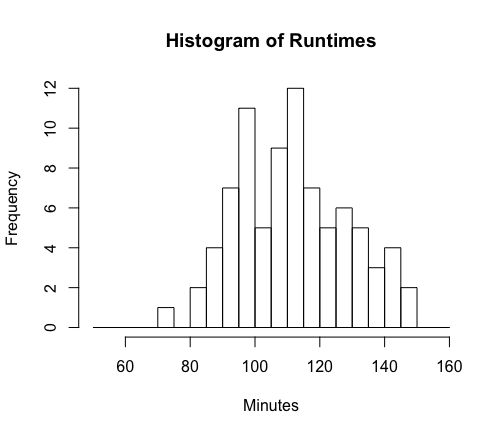
\includegraphics[scale=.5]{PS6c_Holt}
\caption{Ratings v. Rank}
\label{fig:PS6c_Holt}
\end{figure}

\end{document}
